We have conducted two different experiments, one to predict the force measured
by the force sensor and another one to classify the grasp type.
The EMG data were the preprocessed as described in Sec ???.
To assess the performance of the proposed adaptation method we have compared it
to two baseline methods. The first one, \emph{}, consists in using only the old models; the second one, \emph{}, .

\begin{figure}[t]
  \centering
  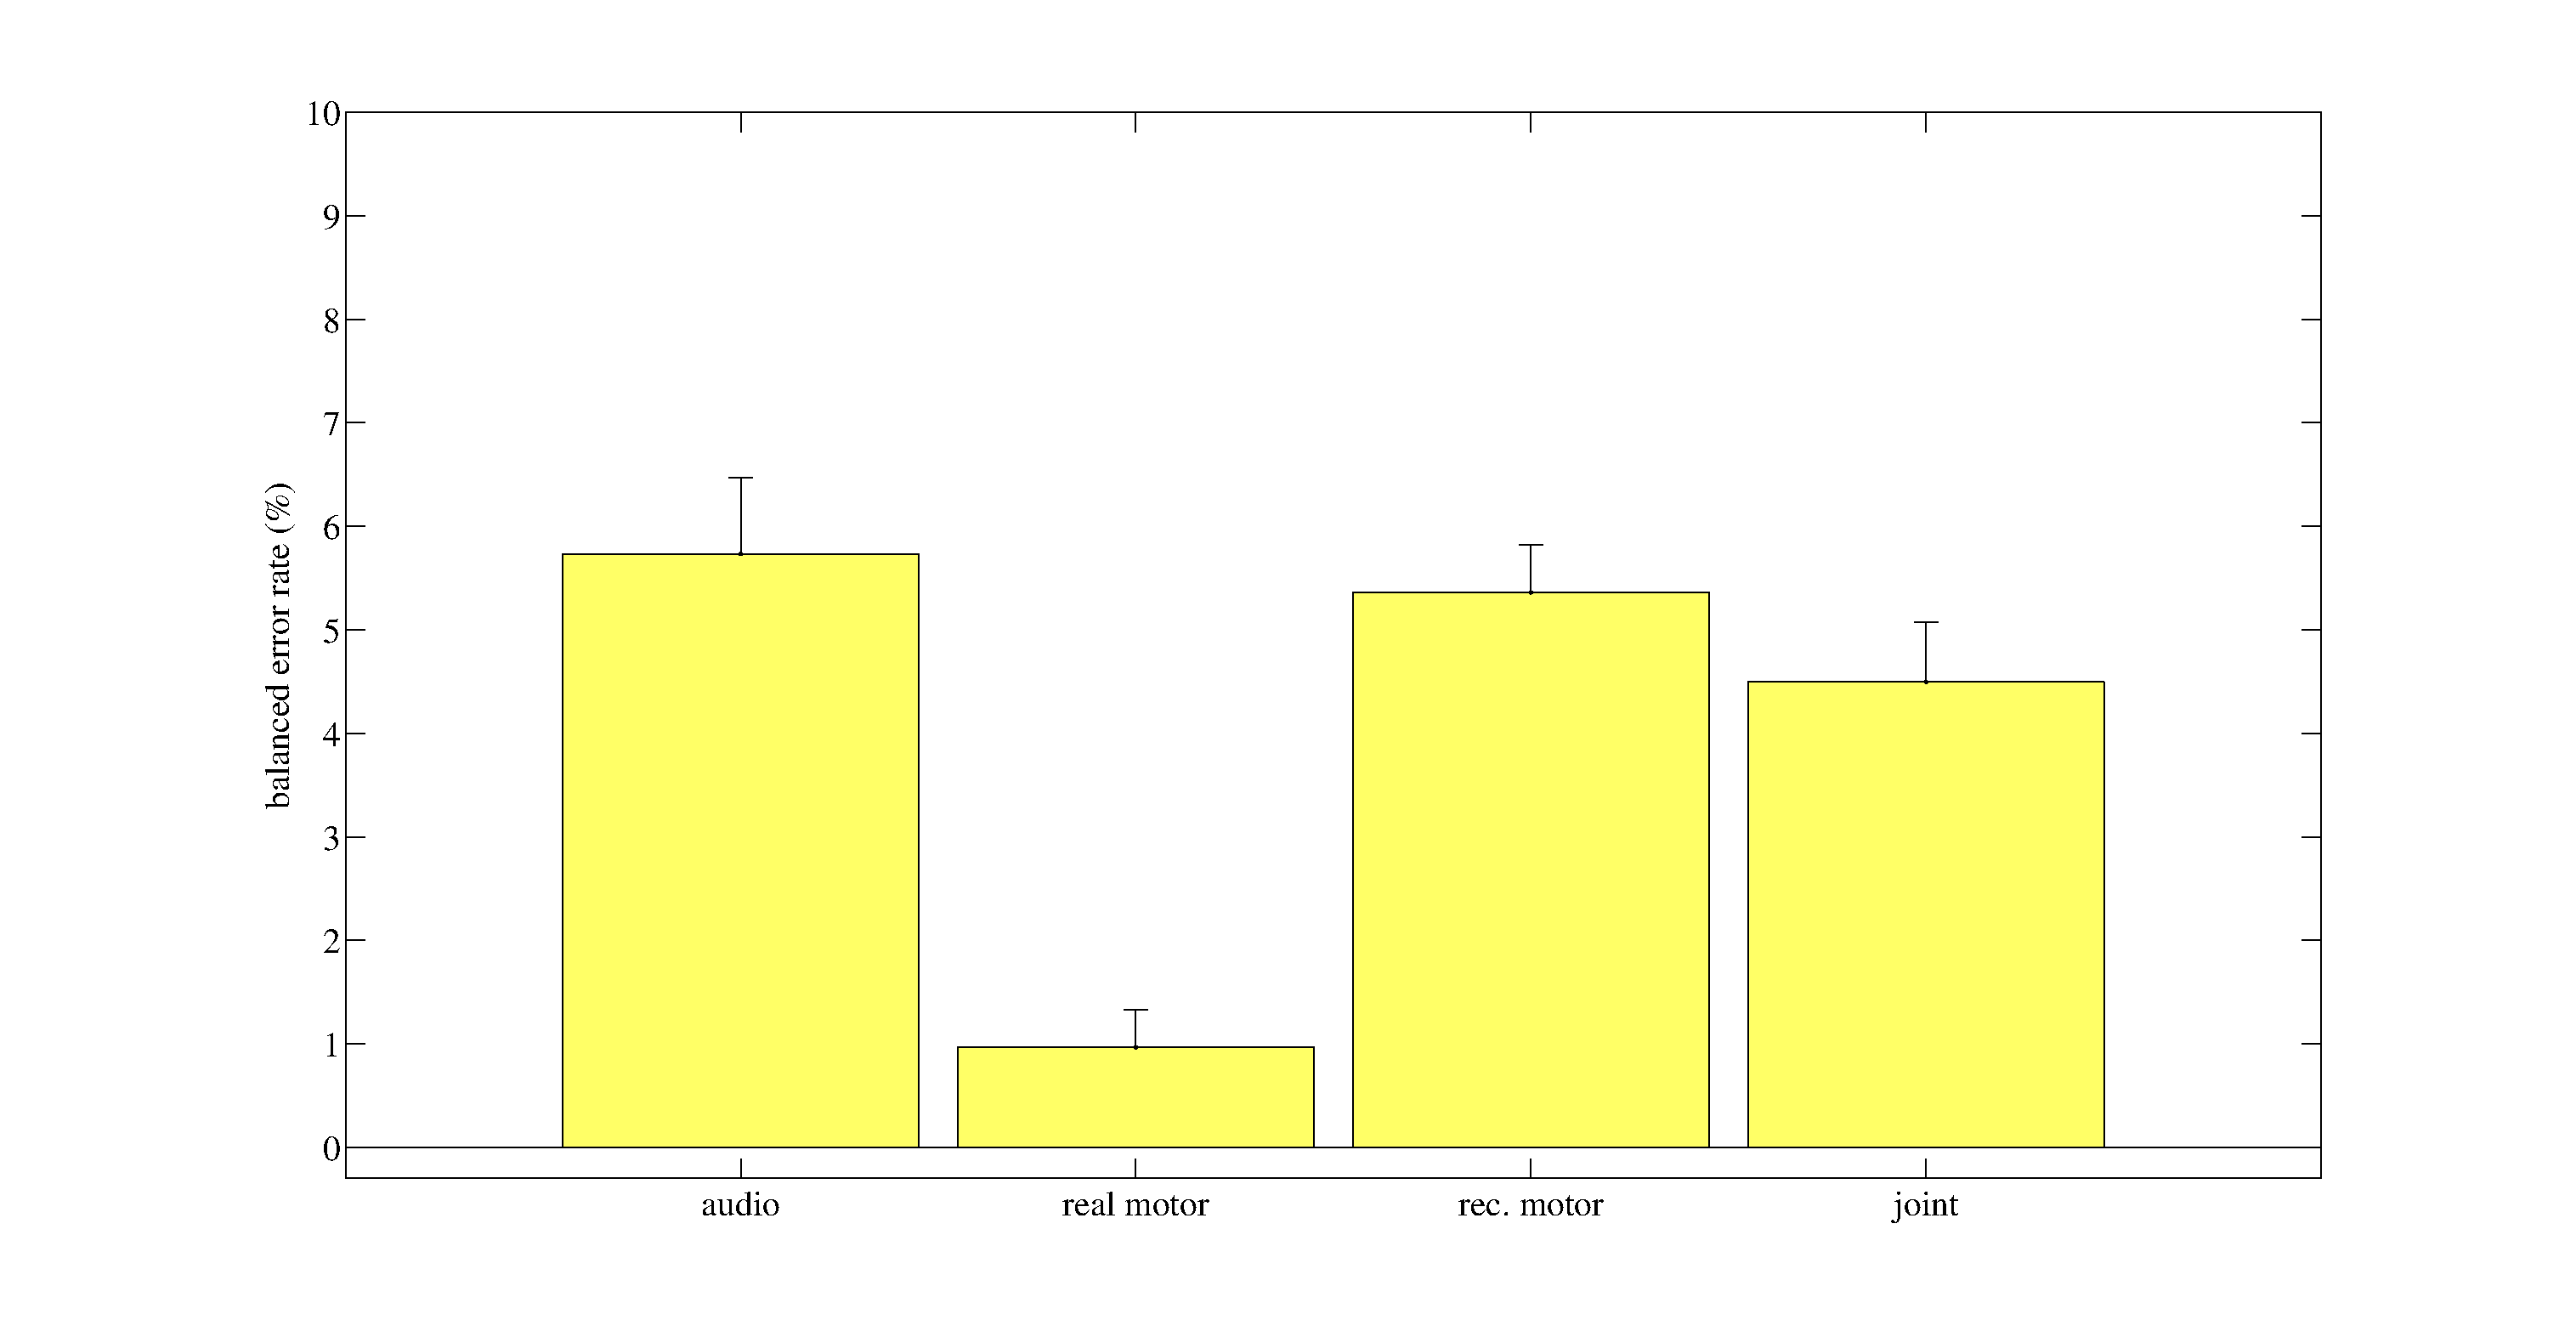
\includegraphics[width=0.95\linewidth]{figs/exp1}
  \caption{The classification experiment.}
  \label{fig:exp1}
\end{figure}

\begin{figure}[t]
  \centering
  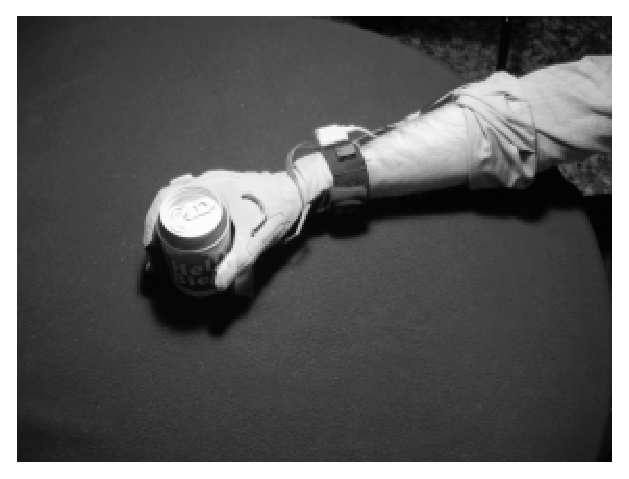
\includegraphics[width=0.95\linewidth]{figs/exp2}
  \caption{The regression experiment.}
  \label{fig:exp2}
\end{figure}